Computing and information systems have become integral to all aspects of our life, and their significance will inevitably continue to increase in the future. Fueled by powerful computing servers, massive storage capacity and unprecedented communication speeds, these systems support an increasingly large number of services and applications, critical to our society, national security and the economy. These applications range from Internet-scale web services, high-performance scientific computing, data-intensive analytics and graph processing, mobile computing for smart distributed environments, to healthcare and disaster management. As our reliance on information technology continues to grow, future infrastructure must support hundreds of thousands, if not millions, of servers, to achieve significantly higher levels of parallelism and handle a massive numbers of storage and communications operations.

The scale needed to address our future computing needs will come at the cost of increasingly sophisticated, complex computing and information systems whose behavior is increasingly difficult to specify, predict and manage.
The upward trend, in terms of scale and complexity, has a direct negative effect on the overall system reliability. 
%The increase in the number of system components significantly increases the propensity of the system to faults, while driving power consumption to unprecedented heights. 
Even with the expected improvement in the reliability of future computing technology, the rate of system level failures will dramatically increase with the number of devices, possibly by several orders of magnitude. This can be clearly seen in Figure~\ref{fig:exe_failure}. For example, a system with 200,000 nodes will experience a mean time between failures (MTBF) of less than one hour, even when the MTBF of an individual node is as large as 5 years. 

\begin{figure}[!t]
	\begin{center}
		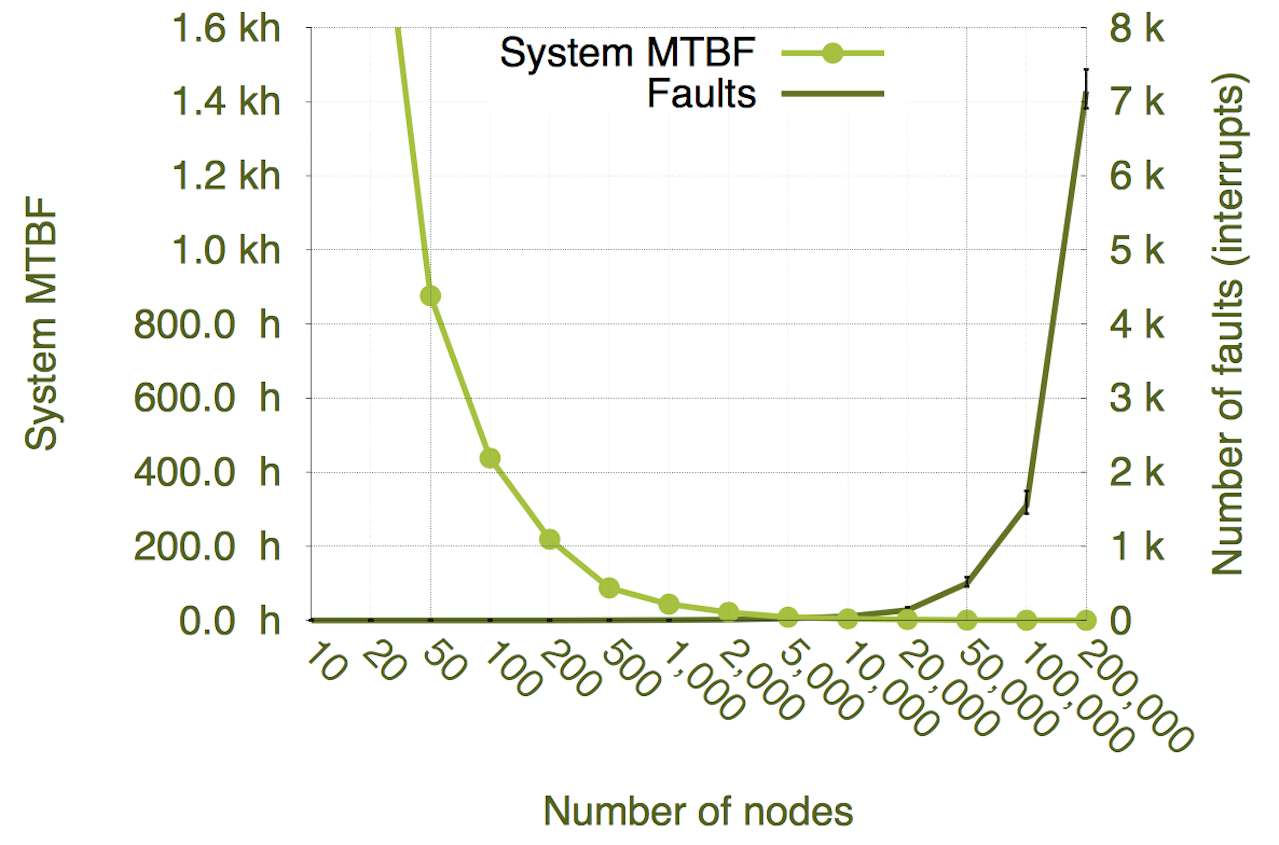
\includegraphics[width=0.9\columnwidth]{Figures/sandia_system_failure_rate_increase_nodes}
	\end{center}
	\vskip -0.25in 
	\caption{Impact of system size on system resilience.}
	\label{fig:exe_failure}
\end{figure}

Another direct consequence of the increase in system scale is the dramatic increase in power requirements. Recent studies show a steady rise in system power consumption to 1-3MW in 2008, followed by a sharp increase to 10-20MW in subsequent years, with the expectation that power consumption could surpass 50MW by 2016~\cite{doe_ascr_exascale_2011}. The US Department of Energy has recognized this trend and established a power limit of 20MW, challenging the research community to provide a 1000x improvement in performance with only a 10x increase in power~\cite{doe_ascr_exascale_2011}. %It is reported in~\cite{elnozahy2003energy} that energy cost in data centers accounts for 23-50\% of the overall expenses, making system power a leading design constraint in future extreme-scale computing infrastructure.
This huge imbalance makes system power a leading design constraint in future extreme-scale computing infrastructure.


Fault tolerance and power management have been studied extensively, although only recently have researchers begun to study the combination of these two competing goals. In today's systems the response to faults mainly consists of restarting the application, including all related software components that have been affected by the fault. To avoid full re-execution of the original task, systems often checkpoint the execution periodically. Upon the occurrence of a hardware or software failure, recovery is then achieved by restarting the computation from a known checkpoint. Given the anticipated increase in system-level failure rates and the time required to checkpoint large-scale compute-intensive and data-intensive applications, it is predicted that, in extreme scale computing environments, the time required to periodically checkpoint an application and restart its execution will approach the system's MTBF. Consequently, applications will make little forward progress, thereby reducing considerably the overall performance of the system~\cite{riesen_sandia_2010}.% Given this limitation, several large-scale application designers avoid checkpointing and rely on re-execution, upon failure, to achieve fault-tolerance. 

More recently, process replication, either full or partial, has been proposed as an alternative to checkpointing, in order to scale to the resilience requirements of large distributed and mission-critical systems~\cite{fiala_2012_sdc,riesen_sandia_2010}. Based on this technique, a process's state and computation are replicated across independent computing
nodes. When the main process fails, one of the replicas takes over the computation task. Replication 
requires at least doubling the number of computing resources, since each process must have at least one replica, thereby 
limiting the system efficiency to 50\%.

There is a delicate interplay between fault tolerance and energy consumption. Checkpointing and replication require additional energy to achieve fault tolerance. Conversely, it has been shown that lowering supply voltages, a commonly used technique to conserve energy, increases the probability of transient faults~\cite{chandra2008defect,zhu2004fail}. The tradeoffs between fault free operation and optimal energy consumption has been explored in the literature. Limited insights have emerged, however, with respect to how adherence to application's desired QoS requirements affects and is affected by the fault tolerance and energy consumption dichotomy. For example, it has been shown that, at scale, coordinated and uncoordinated checkpointing may lead to cascading delays. %Similarly, the overhead of reexcution and replication-based techniques is a dominant factor of the computation and may lead to excessive delay and energy consumption in large-scale computing environments. 
In addition, abrupt and unpredictable changes in system behavior may lead to unexpected fluctuations in performance, which can be detrimental to applications' QoS requirements. The inherent instability of extreme-scale computing systems, in terms of the envisioned high-rate and diversity of their faults, together with the demanding power constraints under which these systems will be designed to operate, calls for a reconsideration of the fault tolerance problem.

To this end, we propose an adaptive and power-aware resilience algorithm, referred to as \textit{Lazy
Shadowing}, as an efficient and scalable alternative to achieve high-levels of resilience, through
forward progress, in extreme-scale, failure-prone computing environments. In the proposed
approach, each process (referred to as main) is associated with a lazy replica (referred to as shadow) to improve resilience. The shadow executes the same code as its
associated main process, but at a reduced CPU rate to save power and energy. %The rate
%at which the shadow runs is derived based on the expected time-to-solution of the supported
%application, the power constraints imposed by the underlying computing infrastructure, and the
%likelihood of failure. 
Upon failure of the main process, the shadow increases its 
execution rate to complete the task, thereby reducing the impact of such a failure on the progress of
the remaining tasks. Successful completion of the main process, however, results in immediate
termination of the shadow. Since the failure rate of an individual component is much lower than that of 
the whole system, it is very likely that, most of the main processes complete their execution
successfully. Consequently, the coupled execution of a main process and its associated shadow 
dramatically increases a power-constrained system's tolerance to failure, at a significantly reduced
energy consumption.

Lazy Shadowing provides a class of stochastically competitive algorithms, which guarantee small relative error with respect to the optimal expected cost, in terms of completion time and energy consumption. One gets different algorithms depending upon the main and shadow processes' execution rates, which are adaptive to the desired balance among the expected completion time of the supported application, the power constraints imposed by the underlying computing infrastructure, and the likelihood of failure. At the same time, we minimize the proposed algorithms' adaptivity to stochastic events by changing the shadow's execution rate only in response to a failure, in order to keep the algorithms simple as well as reduce implementation overhead. 



The rest of the paper is organized as follows. We begin with a survey on related work in Section 
\ref{sec:related_work}. Section \ref{sec:frame_model} defines the Lazy Shadowing 
computational model and Section \ref{frame_multiple} discusses how Lazy Shadowing can be used in 
extreme-scale computing environments for efficient fault tolerance. 
We then introduce three analytical models for performance assessment
in Section \ref{sec:analytical}, 
followed by experiments and evaluation in
section \ref{sec:evaluation}. Section \ref{sec:conclusion} concludes this work and points out 
future research directions.